\documentclass{article}
\usepackage{graphicx}
\usepackage{geometry}
\usepackage{amsmath}
\usepackage{float}
\usepackage{xcolor}
\usepackage{listings}
\usepackage{matlab-prettifier}
\usepackage{caption}
\usepackage{subcaption}
\usepackage{xparse}
\usepackage{hyperref}
\usepackage{amssymb}
\usepackage{verbatim}
\usepackage{fancyhdr}
\pagestyle{fancy}
\usepackage{xspace}
\cfoot{}
\lfoot{Università degli Studi di Padova, Reti di Calcolatori 1, AA 2022-2023}
\rfoot{\thepage}

\newcommand{\Rcerchio}{\textregistered\xspace}

\title{Homework 1\\\textbf{Una semplice tecnica di codifica d'immagini basata sulla DCT}}
\author{Giacomo Calabria - 2007964}
\date{\today}

\begin{document}
    \maketitle
    \section{Introduction}
    L'obiettivo di questo Homework è quello di produrre un programma che effettui una semplice tecnica di codifica basata sulla DCT.\\\\
Il codice fornito è stato scritto nell'ambiente di programmazione MATLAB\Rcerchio in quanto esso dispone della libreria \textit{Image Processing Toolbox} che offre molti strumenti per manipolare ed elaborare in modo semplice le immagini, tra cui comprese la funzione DCT. Inoltre, la possibilità di visualizzare immagini e manipolarle in modo facile e intuitivo è estremamente utile per analizzare e valutare la qualità della codifica effettuata.\\\\
Per eseguire il codice, è necessario salvare l'immagine da elaborare nella stessa cartella del file MATLAB, quindi aprire il file e premere il tasto "Run" o digitare il comando \texttt{"run Project1.m"} nella finestra della console di MATLAB.\\\\
Il codice utilizza alcune funzioni matematiche standard di MATLAB per calcolare il MSE e il PSNR e tracciare le curve del PSNR in funzione di R. E richiede la libreria \textit{Image Processing Toolbox} per gestire l'elaborazione di immagini e in particolare la funzione DCT.\\\\
Il codice richiede l'impostazione di alcuni parametri di input:
\begin{itemize}
    \item Il path/nome del file
    \item Dimensione dei blocchi $N$
    \item La percentuale $R$ di coefficienti DCT da mettere a zero
\end{itemize}
Questi parametri possono essere modificati all'interno del file MATLAB\Rcerchio.

    \clearpage
    \section{Metodo di codifica}
    \begin{enumerate}
    \item Caricamento dell' immagine
    \item Cambio spazio dei colori da RGB a YCbCr
    \item Per ognuna delle componenti Y,Cb e Cr si è proceduto a fare la DCT bidimensionale con blocchi di dimensione $N$ sulla singola componente, utilizzando la funzione \begin{lstlisting}[frame=single,style=Matlab-editor]
blockproc(y, [N N], dctfun);
        \end{lstlisting}dove \texttt{dctfun} è la funzione per la DCT sul blocco.
    \begin{enumerate}
        \item Successivamente è stata calcolata la frazione R\% dei coefficienti DCT dell'\textbf{intera componenete} da mettere a zero 
        \begin{lstlisting}[frame=single,style=Matlab-editor]
perc_y = prctile(abs(y_dct(:)), R);
        \end{lstlisting}
        \item E' stata messa a zero la frazione calcolata al punto precedente \begin{lstlisting}[frame=single,style=Matlab-editor]
y_dct(abs(y_dct) < perc_y) = 0;
        \end{lstlisting}
    \end{enumerate}
    \item E' stata fatta la DCT inversa bidimensionale sui blocchi di lunghezza sempre $N$ sulla singola componente, sempre utilizzando la funzione \begin{lstlisting}[frame=single,style=Matlab-editor]
blockproc(y, [N N], dctinvfun);
        \end{lstlisting} dove \texttt{dctinvfun} è la funzione inversa della DCT sul blocco.
    \item Calcolo dell'\textit{MSE} tra la componente originale e la componente "compressa" \begin{lstlisting}[frame=single,style=Matlab-editor]
mse_y = immse(double(y(:)),double(y_compressed(:)));
    \end{lstlisting}
\end{enumerate}
Successivamente è stato calcolato l'MSE pesato, utilizzando
\begin{equation}
    {MSE}_P = \frac3 4 {MSE}_Y + \frac 1 8 {MSE}_{Cb} + \frac 1 8 {MSE}_{Cr}
\end{equation}
da cui abbiamo calcolato poi il PSNR pesato come
\begin{equation}
    PSNR=10\log_{10} \left(\frac{255^2}{{MSE}_P}\right)
\end{equation}
Abbiamo proceduto poi a plottare in un grafico i diversi valori di PSNR ottenuti facendo variare opportunamente $R$ in un intervallo da 10 a 100.
    \clearpage
    \section{Risultati: grafici del \textit{PSNR}}
    Riportiamo adesso i risultati ottenuti con la tecnica di codifica d'immagine basata su DCT implementata. In Figura \ref{fig:original} è stata riportata l'immagine originale scelta per testare la codifica.
\begin{figure}[H]
    \centering
    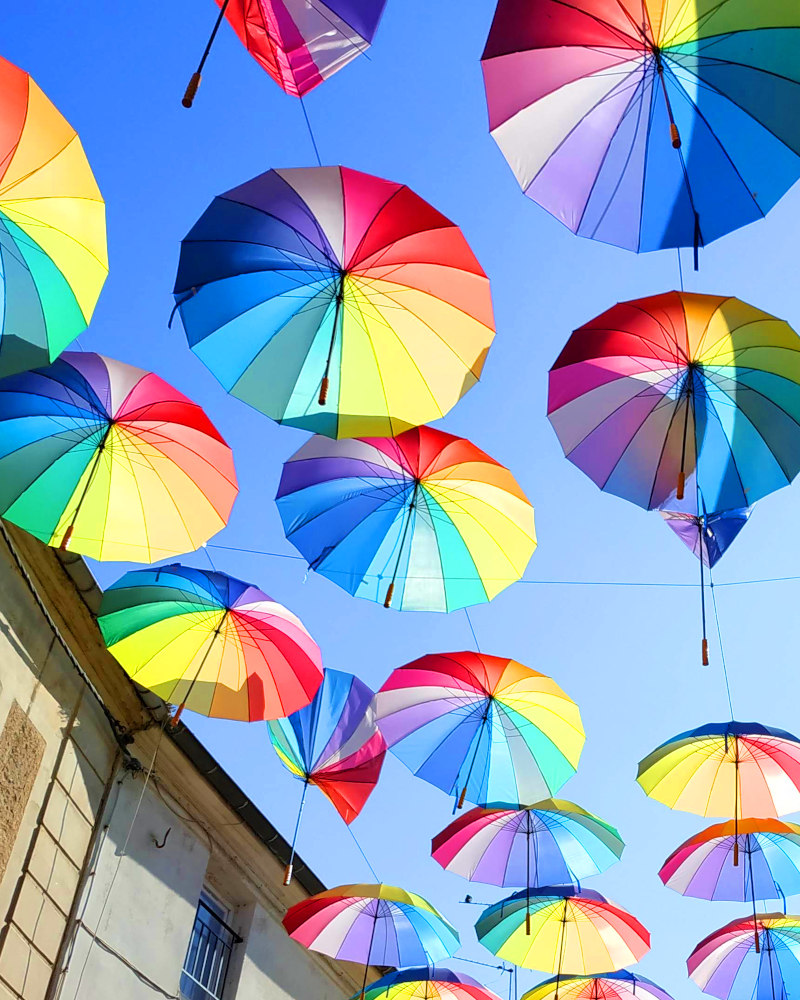
\includegraphics[width=0.65\linewidth]{Original.png}
    \caption{Immagine originale}
    \label{fig:original}
\end{figure}
Dapprima abbiamo tracciato i grafici del PSNR in funzione di $R$ per $N=8,16,64$, facendo variare il parametro $R$ da 10 a 100 in modo lineare a passi di 0.1 in modo da poter apprezzare al meglio l'andamento del grafico. Riportiamo quindi nelle Figure \ref{fig:ris8},\ref{fig:ris16} e \ref{fig:ris64} i grafici.
\begin{figure}[H]
    \centering
    \begin{minipage}{.5\textwidth}
        \centering
	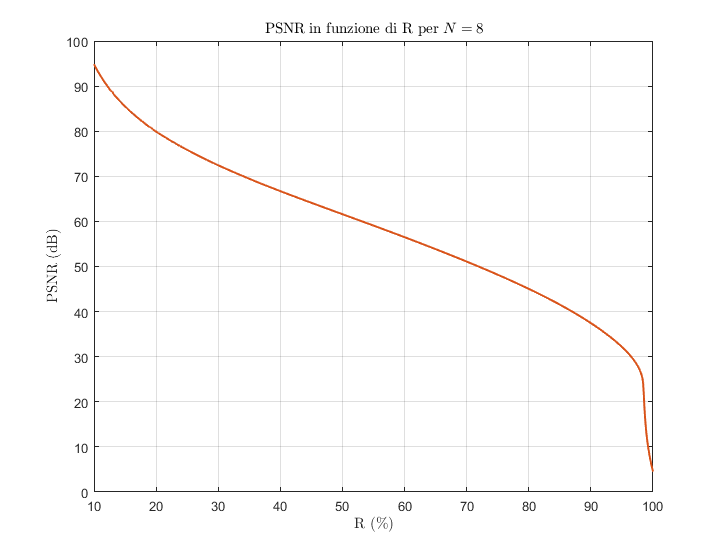
\includegraphics[width=\linewidth]{RIS_N8.png}
	\caption{$N=8$}
	\label{fig:ris8}
    \end{minipage}%
    \begin{minipage}{.5\textwidth}
        \centering
	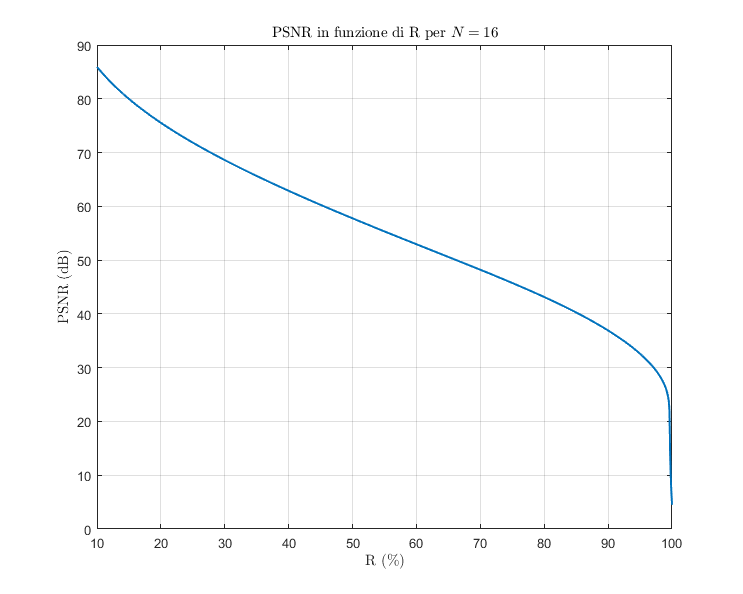
\includegraphics[width=\linewidth]{RIS_N16.png}
	\caption{$N=16$}
	\label{fig:ris16}
    \end{minipage}
\end{figure}
\begin{figure}[H]
	\centering
	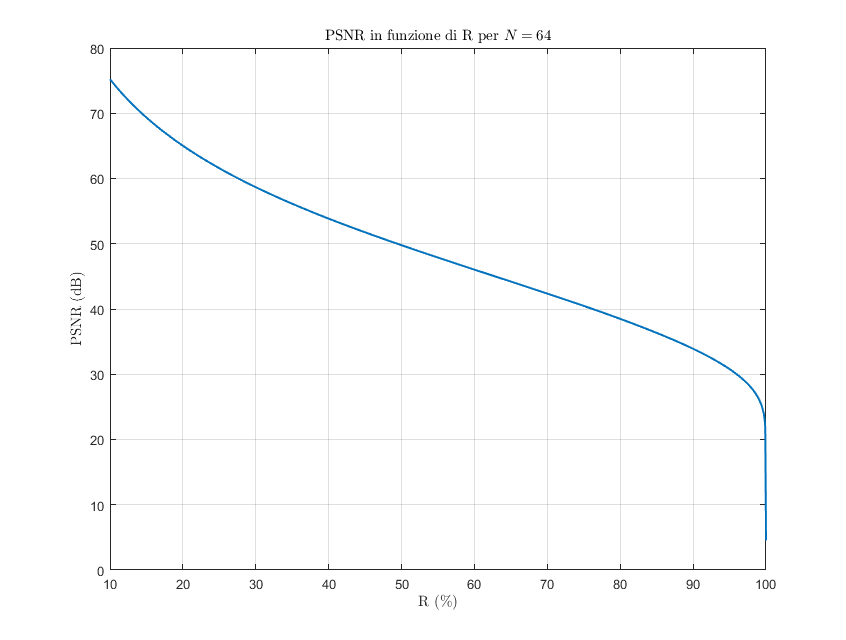
\includegraphics[width=0.75\linewidth]{RIS_N64.png}
	\caption{$N=64$}
	\label{fig:ris64}
\end{figure}
Si è voluto aumentare la "risoluzione" di $R$, rispetto alla consegna, per permettere di vedere il reale andamento del PSNR in funzione di $R$. Viene riportato in Figura \ref{fig:ris} l'andamento del grafico nel caso in cui il parametro $R$ viene fatto variare a passi di 10.
\begin{figure}[H]
	\centering
	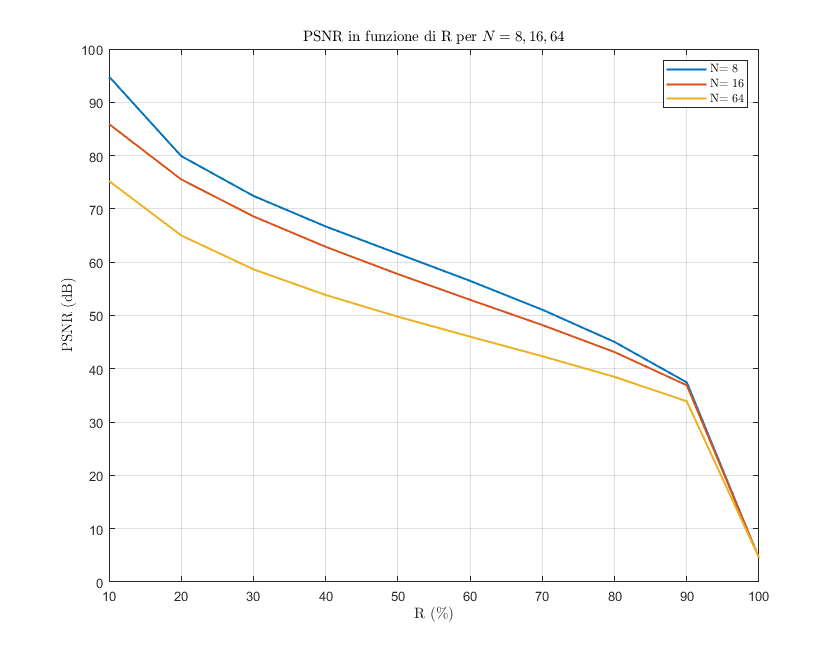
\includegraphics[width=0.7\linewidth]{RIS_TOT.png}
	\caption{Andamento del PSNR per $N=8,16,64$ con passo di $R$ a 10.}
	\label{fig:ris}
\end{figure}
Si osserva che all'aumentare della dimensione dei blocchi la compressione lavora meglio. Questo è dovuto al fatto che con blocchi più grandi è possibile raggruppare più informazioni spaziali in un unico blocco, sono meno sensibili alle variazioni locali dell'immagine, aumentando l'efficacia della codifica DCT. Si nota che per tutti i valori di $N$, il PSNR si riduce rapidamente per valori di $R$ superiori al 90\%\\\\
Si vuole sottolineare infine che il tempo computazionale aumenta sensibilmente diminuendo la dimensione del blocco.
\section{Risultati: immagini codificate}
Infine, riportiamo alcune immagini ricavate dalla nostra codifica, avendo impostato il fattore di compressione $R=98\%$ ad un valore abbastanza elevati per poter apprezzare come l'immagine si degrada a seguito della compressione.\\\\
Si può notare come la qualità dell'immagine compressa peggiora gradualmente all'aumentare della percentuale di coefficienti DCT posti a zero, con una perdita di dettagli e una comparsa di artefatti visibili in alcune zone dell'immagine. Tuttavia, anche quando viene impostata una percentuale elevata $(R>95\%)$, l'immagine compressa rimane abbastanza riconoscibile. Una compressione troppo aggressiva può causare una perdita di informazioni.
\begin{figure}[H]
    \centering
    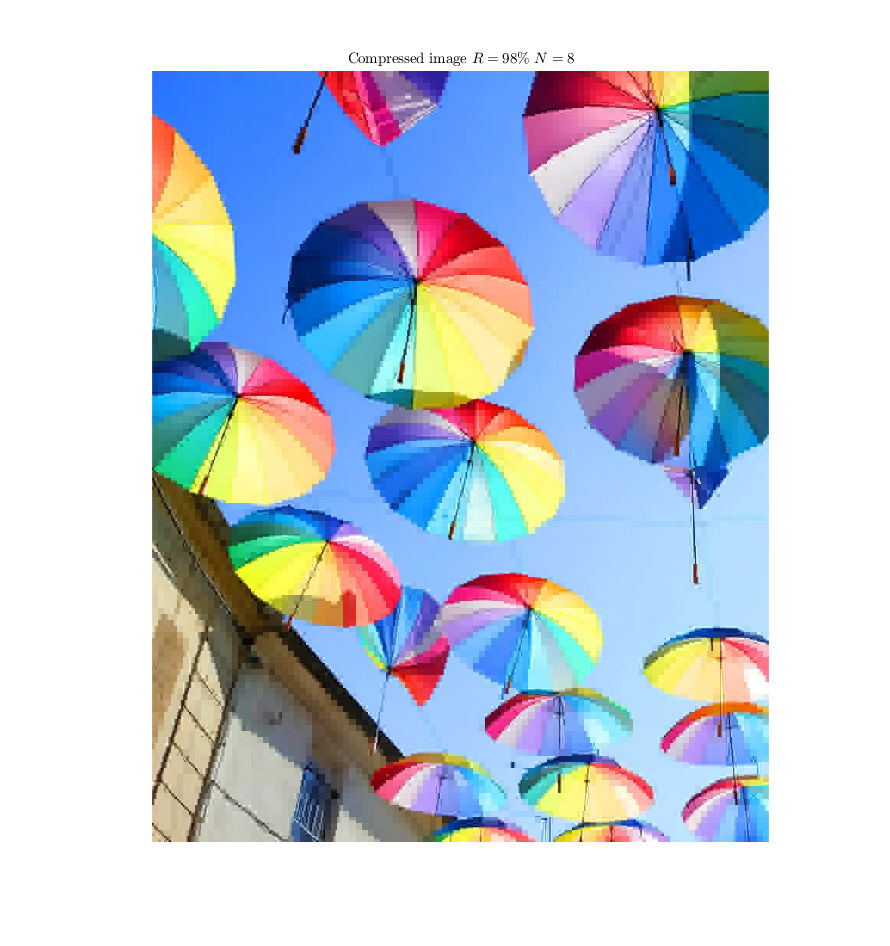
\includegraphics[width=\linewidth]{RIS_N8_R98.png}
    \caption{$N=8,R=98\%,PSNR=26.5859$}
    \label{fig:RIS_N8_R98}
\end{figure}
\begin{figure}[H]
    \centering
    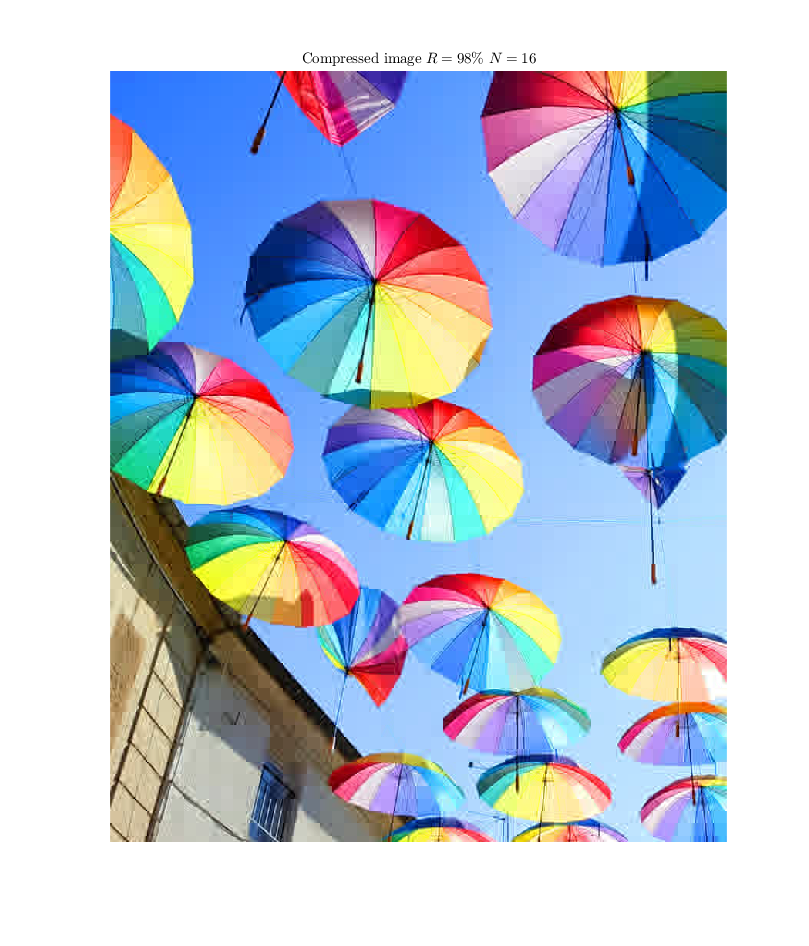
\includegraphics[width=\linewidth]{RIS_N16_R98.png}
    \caption{$N=16,R=98\%,PSNR=28.6002$}
    \label{fig:RIS_N16_R98}
\end{figure}
\begin{figure}[H]
    \centering
    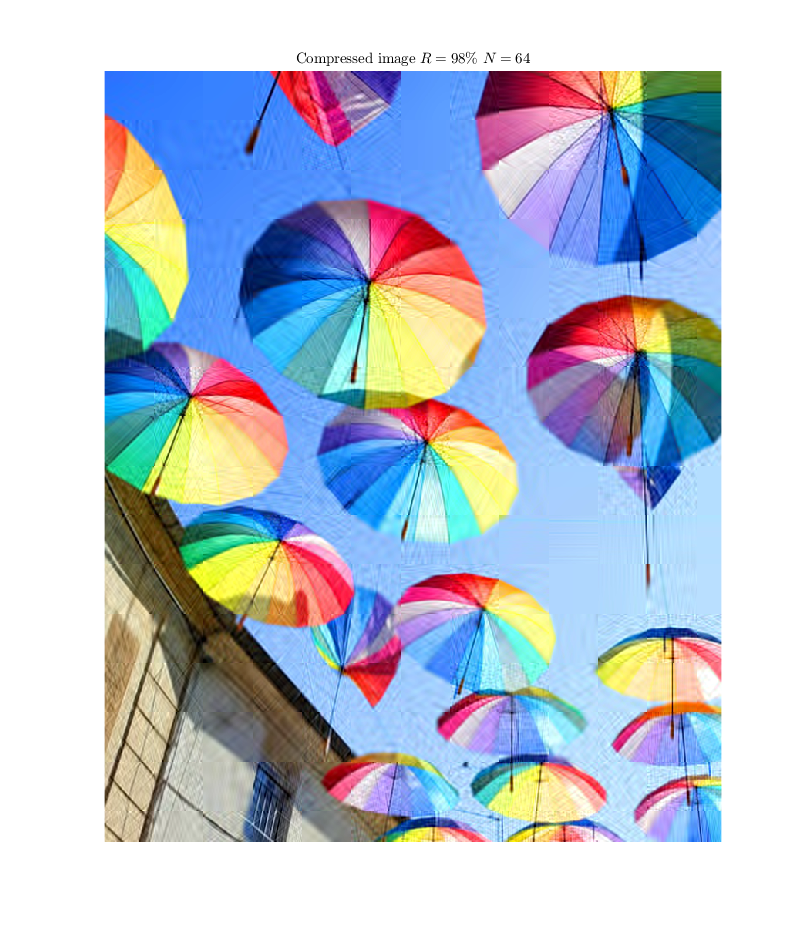
\includegraphics[width=\linewidth]{RIS_N64_R98.png}
    \caption{$N=64,R=98\%,PSNR=27.8918$}
    \label{fig:RIS_N64_R98}
\end{figure}
\end{document}
